\chapter{Заключение}
\section{Постигнати резултати}
Успешно са реализирани ръчно и отдалечено управление на РОБКО 01. Отдалеченото управление се извършва чрез опашка от текстови команди. Управляващите команди могат да се изпращат по интернет и да се четат от файл. Контролерът е способен да управлява всички мотори на робота едновременно и да засича предмети. Разработената система въстановява оригиналната функционалност на РОБКО 01 и демонстрира възможността за отдалечено управление на индустриални роботи. Проектът е демонстриран в предаването "На Кафе" по Нова Телевизия. \cite{na_kafe}
\begin{figure}[!htb]
    \centering
    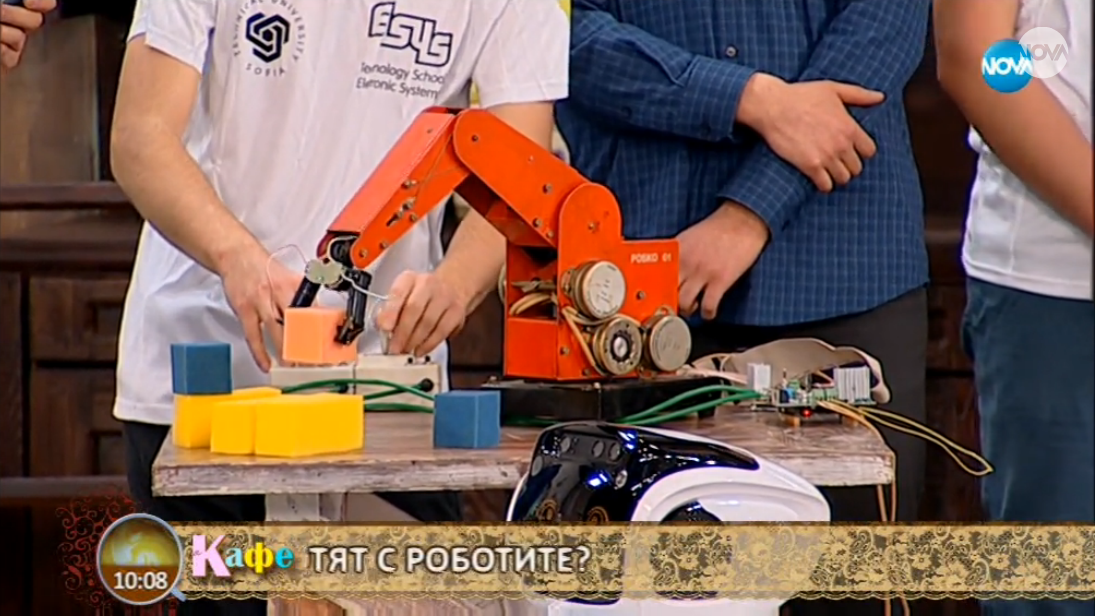
\includegraphics[width=\linewidth]{pictures/na_kafe_s_robko.png}
    \caption{"На Кафе" с туесари}
    \label{fig:na_kafe}
\end{figure}
\section{Бъдещо развитие}
Разработената система страда от известни недостатъци. Командите между клиента и сървъра се изпращат в чист текст. Това позволява подслушване и неоторизиран достъп до управлението на робота. За да се избегне това към комуникационния протокол трябва да се добавят криптиране и аутентикация.\\
\indent{}
Друг съществен проблем е употребата на динамична памет в софтуера на микроконтролера. RAM паметта на микроконтролера е само 128KB и може много лесно да бъде препълнена, дори по невнимание. Когато това се случи има опасност данни да бъдат записани в адреси от паметта, които вече се използват. От този момент нататък поведението на микроконтролера става непредвидимо. Този проблем не може да се отстрани без значителни промени по софтуера, но последствията могат да се ограничат с използването на watchdog модула, който рестартира микроконтролера, ако таймерът му не се нулира периодично.\\
\indent{}
В глава \ref{network_chapter} вече се спомена, че се предвиждат три нови команди. Те ще позволят на робота да запаметява моментната си позиция и да се придвижва до предварително избрани позиции. Голямо подобрение на системата би била способността да изпълнява G код. Това би превърнало РОБКО 01 в CNC машина. Може да се осъществи чрез директно разчитане на G код или чрез преобразуването му в командите, с които работи системата.\\
\indent{}
Сървърната програма може да се разшири за да комуникира с повече от един клиент и с множество контролери. Тези функционалности ще изискват промени и по комуникационния протокол. Интерфейсите на клиентската и сървърната програма също се нуждаят от подобрения. В по-дългосрочен план може да се разработи графична среда.